\chapter{Roboternavigation im Kraftfeld}
\vspace*{-0.2cm}
Die Roboternavigation basierend auf der Potenzialfeldmethode entspricht der Bewegung eines Körpers im \textit{Kraftfeld} des Potenzialfelds.

\vspace*{-0.1cm}
\section{Berechnung der Gradienten}
\enlargethispage{0.9cm}

Das Kraftfeld entspricht dem negativen Gradientenfeld des Potenzialfelds \cite{khatib.1985}. Auf jede Koordinate wirkt eine Kraft $F_{x/y/rotation}(\texttt{x}, \texttt{y}, \texttt{rotation})$ in Höhe der negativen Potentialänderung, zerlegt in die drei kartesischen Komponenten des Konfigurationsraums:
\vspace*{0.13cm}
\begin{equation*}
 F_{x}(\texttt{x}, \texttt{y}, \texttt{rotation}), F_{y}(\texttt{x}, \texttt{y}, \texttt{rotation}), F_{rotation}(\texttt{x}, \texttt{y}, \texttt{rotation}) = -\nabla U(\texttt{x}, \texttt{y}, \texttt{rotation})
\end{equation*}

Um die Gradienten zwischen dem letzten Rotationszustand und $0$° zu berechnen, wird die erste und letzte Rotationsebene an das jeweils andere Ende der Dimension \texttt{potential[rotation]} kopiert:
\vspace*{0.15cm}
\begin{equation*}
\hspace*{-0.0075\linewidth}
\resizebox{1.05\linewidth}{!}{
$
	\texttt{potential\_padded} = \texttt{np.concatenate([potential[rotations-1], potential, potential[0]])}
$
}
\hspace*{-0.0075\linewidth}
\end{equation*}


Die kopierten Rotationsebenen werden nach Berechnung der Kraftfelder entfernt:
\vspace*{0.13cm}
\begin{equation*}
\hspace*{-0.1\linewidth}
\resizebox{1.2\linewidth}{!}{
$
\texttt{force\_field\_rotation}, \texttt{ force\_field\_y}, \texttt{ force\_field\_x} = -\texttt{np.gradients(potential\_padded)[1 : rotations-1]}
$
}
\hspace*{-0.1\linewidth}
\end{equation*}

Somit entspricht $\texttt{force\_field\_rotation[rotations-1]} > 0 $ einer Kraft in Richtung $\texttt{force\_field\_rotation[0]}$ und $ \texttt{force\_field\_rotation[0]} < 0 $ entspricht einer Kraft in Richtung $\texttt{force\_field\_rotation[rotations-1]}$.
\begin{figure}[H]
	\centering
	\footnotesize
	\centerline{\resizebox{0.63\linewidth}{!}{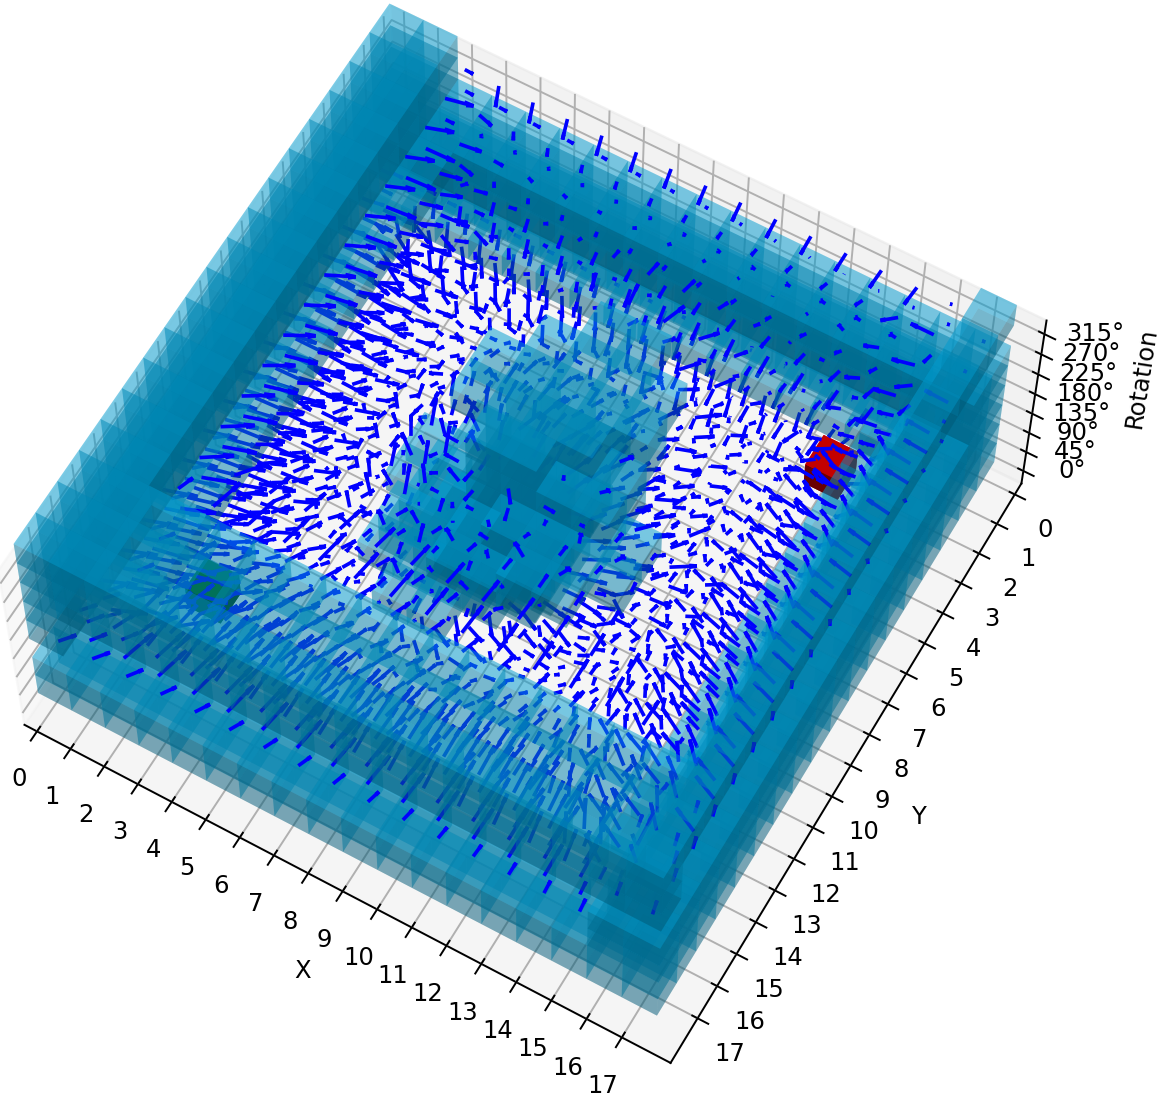
\includegraphics{bilder/force-field.png}}}
	\vspace*{-0.23cm}
	\caption{Darstellung des negativen Gradientenfelds als Kraftpfeile im Konfigurationsraum.}
\end{figure}

\subsection{Gradienten an Grenzen und Hindernissen}

Um die Grenzen des Konfigurationsraums einzuhalten, werden unzulässige Kräfte an den X- und Y-Grenzen auf $0$ gesetzt. Durch dieses manuelle Abschneiden der Kräfte können an den Grenzen lokale Minima entstehen.
\begin{figure}[H]
	\centering
	\footnotesize
	\centerline{\resizebox{0.65\linewidth}{!}{\input{bilder/gradient-clipping_latex.pdf_tex}}}
	\caption{Das Setzen der Gradienten in Grenznähe auf $0$ kann zu lokalen Minima führen.}
\end{figure}
\vspace*{-0.1cm}
Im Numpy Potenzialfeld \texttt{potential} haben Hindernisse das Potenzial \texttt{np.nan}. Somit berechnet \texttt{np.gradients()} für jede an ein Hindernis grenzende Koordinate den Gradienten \texttt{np.nan}.
Um die Kräfte an Hindernissen analog zu Kräften an den Grenzen des Konfigurationsraums zu interpretieren, müssen diese manuell berechnet werden. 
Sollte die berechnete Kraft einer Dimension in Richtung des Hindernisses zeigen, wird diese ebenfalls auf $0$ gesetzt. Nachfolgende Tabelle zeigt dies beispielhaft für Hindernisse im Kraftfeld der X-Achse \texttt{force\_field\_x}:
\begin{table}[H]
\centerline{\resizebox{0.9\linewidth}{!}{
\begin{tabular}{|c|c|c|}
\hline
\textbf{Koordinate Hindernis}                                                & \textbf{\texttt{force\_field\_x[rotation][y][x] = -1*...}}                                                        & \textbf{\texttt{= 0}, wenn ...} \\ \hline
$x+1$ (rechts)                                                               & \texttt{potential[z, y, x] - potential[z, y, x-1]} & $<0$                               \\ \hline
$x-1$ (links)                                                                & \texttt{potential[z, y, x+1] - potential[z, y, x]} & $>0$                                \\ \hline
\begin{tabular}[c]{@{}c@{}}$x+1$ und $x-1$\\ (rechts und links)\end{tabular} & \texttt{0}                                                                           & N/A                                 \\ \hline
\end{tabular}}}
\end{table}
Wird die Kraft einer Dimension auf $0$ gesetzt, wobei die Kräfte der anderen Kraftfelder an dieser Koordinate ebenfalls $0$ sind, entsteht ein lokales Minimum oder Plateau.

\subsection{Behandlung lokaler Maxima}

Im Unterschied zu einem lokalen Minimum oder Plateau ist bei einem lokalen Maximum das Potenzial der Nachbarn streng monoton niedriger als das der aktuellen Koordinate.
In diesen Fällen wird zu einem der beiden Nachbarn ein künstliches Hindernis gesetzt und der Gradient neu berechnet.
\begin{figure}[H]
	\centering
	\footnotesize
	\centerline{\resizebox{0.9\linewidth}{!}{\input{bilder/local-maxima_latex.pdf_tex}}}
	\caption{Lokale Maxima können durch künstliche Hindernisse behoben werden.}
\end{figure}


\section{Gradientenabstieg}

Die berechneten Gradientenfelder ermöglichen die Roboternavigation mit dem \textit{Gradientenabstiegsverfahren}. Pro Verarbeitungsschritt wird die nächste Koordinate basierend auf der betragsmäßig größten Kraft in $F_{x}(\texttt{x}, \texttt{y}, \texttt{rotation})$, $F_{y}(\texttt{x}, \texttt{y}, \texttt{rotation})$ und $F_{rotation}(\texttt{x}, \texttt{y}, \texttt{rotation})$ gewählt, bis eine bereits besuchte Koordinate oder eine Koordinate mit Kräftegleichgewicht $F_{x}(\texttt{x}, \texttt{y}, \texttt{rotation}) = F_{y}(\texttt{x}, \texttt{y}, \texttt{rotation}) = F_{rotation}(\texttt{x}, \texttt{y}, \texttt{rotation}) = 0$ erreicht wird:

\begin{algorithm}
\caption{Gradientenabstiegsverfahren}
\begin{algorithmic}[1]
    \State \textbf{Initialisierung:}
    \State \hspace{\algorithmicindent} $(\texttt{x}_{\text{current}}, \texttt{y}_{\text{current}}, \texttt{rotation}_{\text{current}}) = \texttt{start\_point}$
    \State \hspace{\algorithmicindent} Visited $V \leftarrow \emptyset$
	\vspace*{0.3cm}
    \While{true}
        \If{$(\texttt{x}_{\text{current}}, \texttt{y}_{\text{current}}, \texttt{rotation}_{\text{current}}) = \texttt{goal\_point}$}
            \State \textbf{return} Ziel gefunden
        \EndIf
		\vspace*{0.1cm}
        \State $\texttt{force\_field\_x/y/rotation}\texttt{[}\texttt{rotation}_{\text{current}}\texttt{][}\texttt{y}_{\text{current}}\texttt{][}\texttt{x}_{\text{current}}\texttt{]} = 0$
        \State $(\texttt{dx}, \texttt{dy}, \texttt{drotation}) \gets \max(|\texttt{force\_field\_x/y/rotation}\texttt{[}\texttt{rotation}_{\text{current}}\texttt{][}\texttt{y}_{\text{current}}\texttt{][}\texttt{x}_{\text{current}}\texttt{]}|)$
		\vspace*{-0.3cm}
        \If{$(\texttt{dx}, \texttt{dy}, \texttt{drotation}) = (0,0,0)$}
            \State \textbf{return} Lokales Minimum oder Plateau
        \EndIf
     	\vspace*{0.1cm}
        \State $(\texttt{x}_{\text{current}}, \texttt{y}_{\text{current}}, \texttt{rotation}_{\text{current}}) \gets (\texttt{x}_{\text{current}} + \texttt{dx}, \texttt{y}_{\text{current}} + \texttt{dy}, \texttt{rotation}_{\text{current}} + \texttt{drotation})$
		\vspace*{-0.3cm}
        \If{$(\texttt{x}_{\text{current}}, \texttt{y}_{\text{current}}, \texttt{rotation}_{\text{current}}) \in V$}
            \State \textbf{return} Lokales Minimum
		\Else
			\State $(\texttt{x}_{\text{current}}, \texttt{y}_{\text{current}}, \texttt{rotation}_{\text{current}}) \rightarrow V$
        \EndIf
    \EndWhile
\end{algorithmic}
\end{algorithm}

Gemäß der in Kapitel \ref{ch:roboterbewegung} definierten Roboterbewegungen darf pro Verarbeitungsschritt nur eine Translation um eine Einheit entlang der Dimensionen des Konfigurationsraums  durchgeführt werden: $ (\texttt{dx}, \texttt{dy}, \texttt{drotation}) \in \{(\texttt{1},\texttt{0},\texttt{0})(\texttt{-1},\texttt{0},\texttt{0}),(\texttt{0},\texttt{1},\texttt{0}),(\texttt{0},\texttt{-1},\texttt{0}),(\texttt{0},\texttt{0},\texttt{1}),(\texttt{0},\texttt{0},\texttt{-1})\}$
\vspace*{0.1cm}
\begin{figure}[h!]
	\centering
	\footnotesize
	\centerline{\resizebox{1\linewidth}{!}{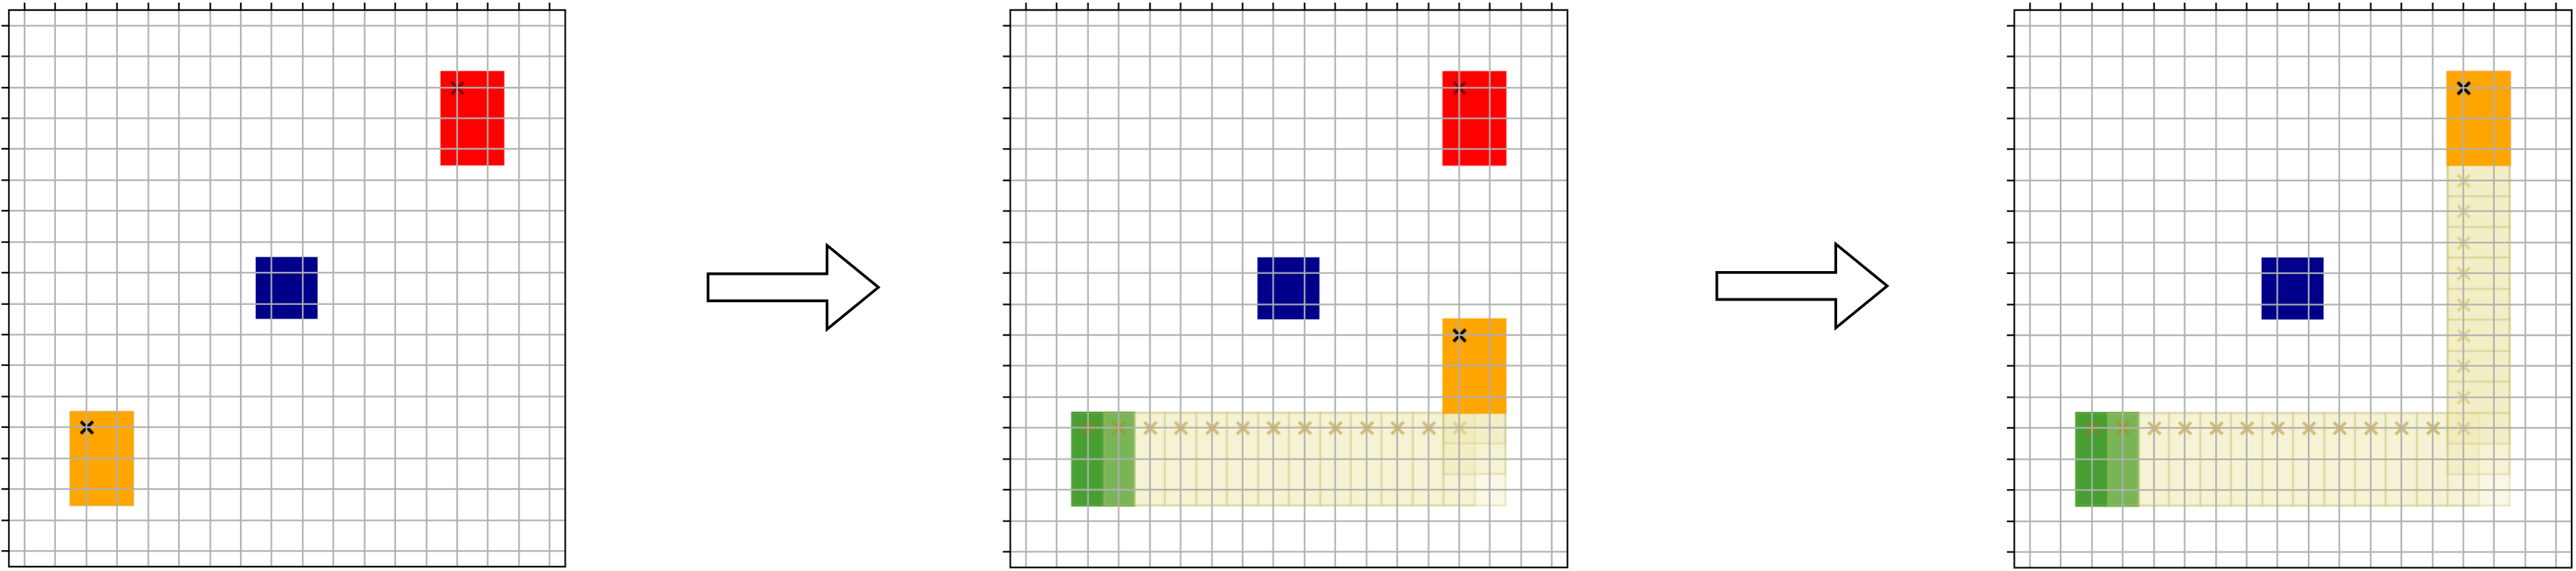
\includegraphics{bilder/grad-desc.png}}}
	\caption{Roboternavigation über das Gradientenabstiegsverfahren im Kraftfeld des Wavefront-Potenzialfelds.}
\end{figure}




